\begin{figure}[t!]
\centering
\begin{subfigure}{.23\textwidth}
  \centering
  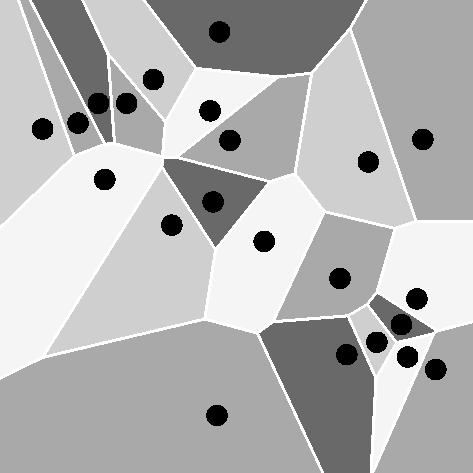
\includegraphics[width=\linewidth]{figure2_a.pdf}
\end{subfigure}\hfill
\begin{subfigure}{.23\textwidth}
  \centering
  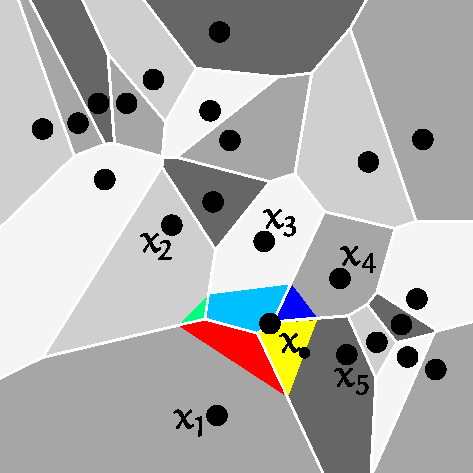
\includegraphics[width=\linewidth]{figure2_b.pdf}
\end{subfigure}\hfill
\begin{subfigure}{.23\textwidth}
  \centering
  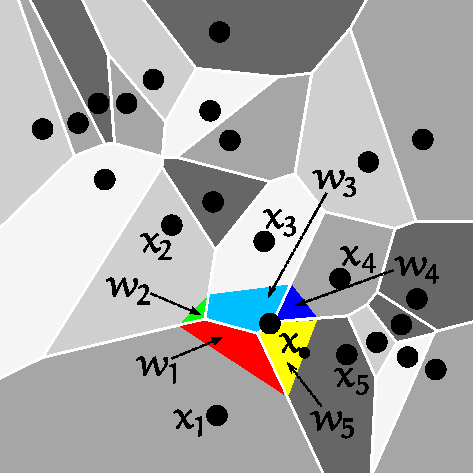
\includegraphics[width=\linewidth]{figure2_c.pdf}
\end{subfigure}\hfill
\begin{subfigure}{.23\textwidth}
  \centering
  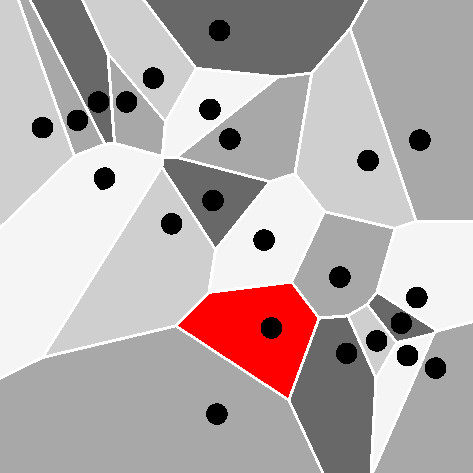
\includegraphics[width=\linewidth]{figure2_d.pdf}
\end{subfigure}
\caption{From \textit{left} to \textit{right}: Clipped tessellation. For other manifolds the curvature should be considered; Tessellation with added point creates a new Voronoi region \textit{stealing} area from the neighboring regions; The determined weights by the fractional amount of occupied area; Tessellation with added point.}
\label{fig:voronoi}
\end{figure}
